%==============================================================================
% figures/F17_spectral_by_period_placeholder.tex --- Implementation placeholder
%==============================================================================
% Required source CSV: results/F17_spectral_by_period.csv
% Required columns: period, theta_1, theta_2, theta_3, weight, stress_flag
% Replacement instruction: generate a PDF with this basename and replace this
% tikzpicture by an includegraphics command, preserving caption and label.
%==============================================================================
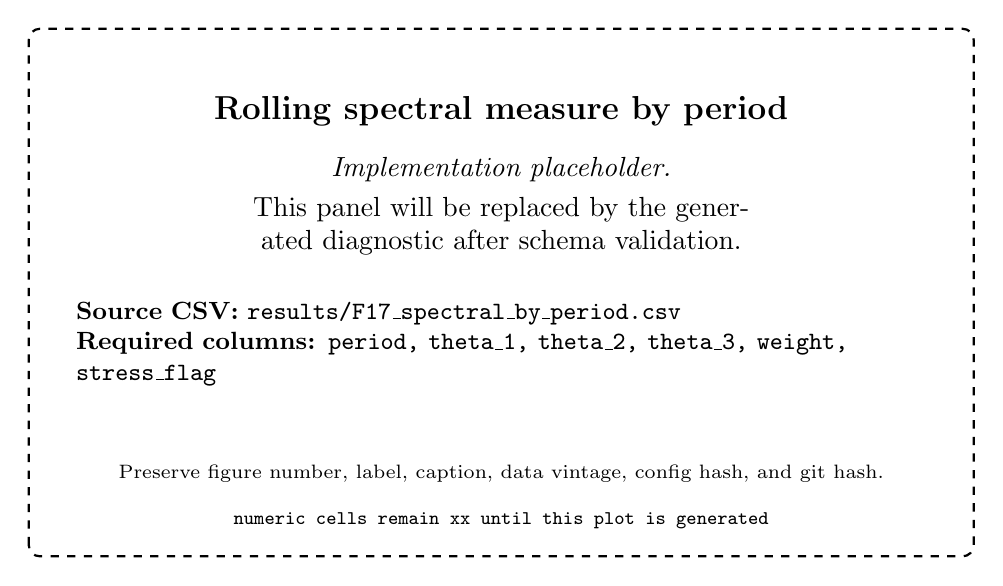
\begin{tikzpicture}
\draw[thick, dashed, rounded corners] (0,0) rectangle (12,6.7);
\node[align=center, font=\large] at (6,5.65) {\textbf{Rolling spectral measure by period}};
\node[align=center, text width=10.6cm] at (6,4.45) {\emph{Implementation placeholder.}\\[0.25em]
This panel will be replaced by the generated diagnostic after schema validation.};
\node[align=left, text width=10.8cm, font=\small] at (6,2.7) {\textbf{Source CSV:} \texttt{results/F17\_spectral\_by\_period.csv}\\
\textbf{Required columns:} \texttt{period, theta\_1, theta\_2, theta\_3, weight, stress\_flag}};
\node[align=center, font=\scriptsize] at (6,1.05) {Preserve figure number, label, caption, data vintage, config hash, and git hash.};
\node[align=center, font=\scriptsize\ttfamily] at (6,0.45) {numeric cells remain xx until this plot is generated};
\end{tikzpicture}
